\chapter{Event Reconstruction and simulation}
\label{CHAPTER:EventReconstructionAndSimulation}

\glsresetall % Resetting all acronyms

This chapter describes how the \gls{CMS} detector produces physics objects from the information collected at each event. The \glsreset{VBF} Higgs to invisible analysis uses almost all the physics objects produced by the detector and for this uses information from all the experiment sub-detectors. The following sections detail for each of these objects how they are reconstructed and what are the choices made to filter them.

%%%%%%%%%%%%%%%%%%%%%%%%%%%%%%%%%%%%%%%%%%%%%%%%%%%%%%%%%%%%%%%%%%%%%%%%%%%%%%%%%%%%%%%
%%% SECTION
%%%%%%%%%%%%%%%%%%%%%%%%%%%%%%%%%%%%%%%%%%%%%%%%%%%%%%%%%%%%%%%%%%%%%%%%%%%%%%%%%%%%%%%
\section{Tracks}
\label{SECTION:EventReconstructionAndSimulation_Tracks}

%Status: DONE

Reconstructing the trajectories of charged particles allows us to measure their momentum and determining their charge. This is possible by analysing the hit patterns in the inner tracking system. In \gls{CMS} this reconstruction is made with the \gls{CTF} algorithm \cite{ARTICLE:CMSTrackReconstruction}. The relevant steps for track generation are described below:

\begin{itemize}
  \item Seed generation is made with hits at the pixel detector. A track seeds can be made with two or three hits. In the first case a know vertex or the beam spot is used to constrain the seed momentum. The parameters of each seed are estimated using the assumption that the trajectory is a helix, but it takes into account hit errors and multiple scattering \cite{ARTICLE:CMSTrackReconstructionSeedGeneration}.
  \item The track seed is extrapolated through the tracker layers with on a combinatorial Kalman filter \cite{ARTICLE:KalmanFilteringTrackVertexFitting} . For each additional layer, the best matching hit if any is added and track parameters are recomputed. This procedure continues until the last layer is reached \cite{ARTICLE:CMSTrackReconstruction}.
  \item Ambiguity resolution may be necessary since since it is possible to have the same track being reconstructed from different seeds, or a seed may results in more than a single trajectory candidate. The resolve this possible double counting, when considering a pair of tracks with more than 50\% of shared hits, we discard the one with less hits. In case so equal number of hits the one with lowest $\chi^2$ is kept. 
  \item After the track building and cleaning stage is done final refitting is performed. This procedure is aimed at removing possible bias by constrains at the seed forming stage. A standard Kalman filter and smoother are used.
\end{itemize}

The process of track finding is repeated up to six times where the hits for each successfully reconstructed track are removed for the next iteration. Using early \gls{LHC} data and a dataset of pions and muons it was possible to estimate that the tracking efficiency is $>98\%$ for all track $\pt > 500\,\MeV$ and $>99\%$ for tracks with $\pt > 2,\GeV$ \cite{ARTICLE:CMSMeasurmentTrackEfficiency}.

%%%%%%%%%%%%%%%%%%%%%%%%%%%%%%%%%%%%%%%%%%%%%%%%%%%%%%%%%%%%%%%%%%%%%%%%%%%%%%%%%%%%%%%
%%% SECTION
%%%%%%%%%%%%%%%%%%%%%%%%%%%%%%%%%%%%%%%%%%%%%%%%%%%%%%%%%%%%%%%%%%%%%%%%%%%%%%%%%%%%%%%
\section{Vertex Reconstruction}
\label{SECTION:EventReconstructionAndSimulation_Vertex}

%Status: DONE

The \gls{LHC} can produce extreme collision intensities which are obtained partially by having multiple collisions happening at each bunch crossing. As it has been discussed in section \ref{SUBSECTION:ExperimentalApparatus_CMS_RunningAndPerformance} an average of 21 simultaneous collisions happened per bunch crossing in the \gls{CMS} experiment during 2012. In this environment, it is crucial to identify the \gls{PV} and the particles that come from it. This information can then be used to reject particles coming from other additional collisions and to identify displaced vertices which can be the signature of long lived particles like b-mesons.

The individual tracks are reconstructed making use of the inner tracker. Each vertex is initially seeded by two tracks with separation in \textit{z} less than $1\,\centi\meter$. Then remaining track are clustered to seed vertex with the \gls{DA} algorithm \cite{ARTICLE:DeterministicAnnealing}. After the clustering process is done, the position of each vertex is recomputed using the adaptive vertex fitter algorithm \cite{ARTICLE:AdaptiveVertexFitting}. In this algorithm weights, $w_{i}$ are assigned to each track according to how compatible they are with the fitted vertex position. Weight vary from 1 to 0, being that track assigned weights of close 1 are highly compatible with the vertex and close 0 would be given to low compatibility tracks. Then we can define the number of degrees of freedom of the new fit as:

\begin{equation}
n_{dof}(vertex)=2\sum\limits_{i}^{tracks} w_i - 3
\end{equation}

This variable can be used to distinguish real proton-proton interactions from misclustered vertices, since it is correlated with the number of tracks compatible with that specific vertex \cite{ARTICLE:CMSTrackingAndPrimaryVertex}. The vertex position and resolution have been measured with \gls{LHC} data and compared with simulation. The resulting plots can be found in figure \ref{FIGURE:EventReconstructionAndSimulation_Vertex} as a function of number of tracks.

\begin{figure}[htp]%
\centering
\subfloat[][]{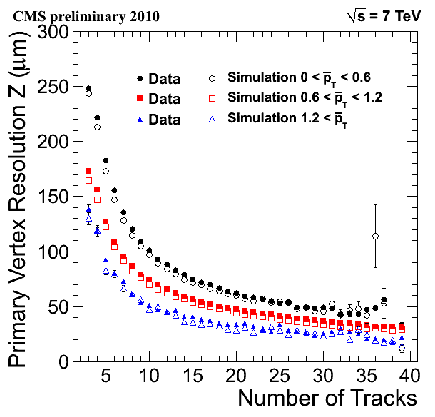
\includegraphics[width=0.45\linewidth]{Chapter04/Vertex/Images/vtx-res.pdf}}\qquad
\subfloat[][]{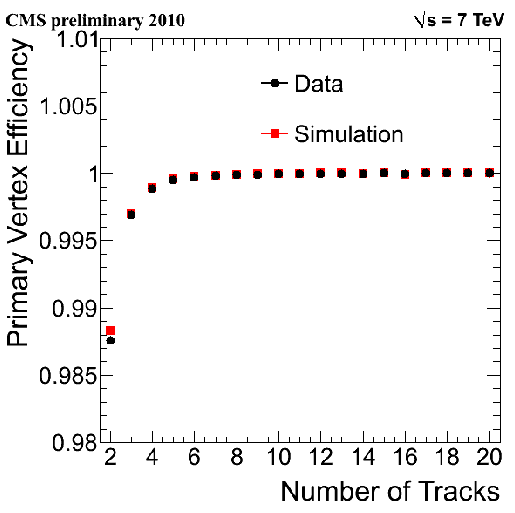
\includegraphics[width=0.45\linewidth]{Chapter04/Vertex/Images/vtx-eff.pdf}}\\
\caption[Primary vertex resolution in the $z$ coordinate and vertex reconstruction efficiency as a function of the number of constituent tracks.]{(a) Primary vertex resolution in the $z$ coordinate a function of the number of associated tracks. Results are give for three ranges of average track \pt. (b) Primary vertex efficiency as a function of the number of associated track \cite{ARTICLE:CMSTrackingAndPrimaryVertex}}
\label{FIGURE:EventReconstructionAndSimulation_Vertex}
\end{figure}

The \gls{PV} is defined as the vertex with highest sum of associated tracks \pt squared. In situations were no vertex can be reconstructed, like if there is a tracking failure, the beam spot position is assumed. Knowing precisely the interaction point allows to determine particle candidate quantities relative to it which allow for better object identification and pile-up control. 

Most \gls{CMS} analysis, including the ones presented in this thesis, require explicitly that a good vertex is reconstructed with the following characteristics:

\begin{itemize}
  \item We require a real reconstructed vertex from tracks, not the beam spot.
  \item A minimum number of degrees of freedom: $n_{dof}>4$.
  \item Collision must be near the interaction point. We require longitudinal distance to be $|z|<=24\,\centi\meter$.
  \item We required the collision be be close to the beam line. Radial distance to beam line: $d_{xy}<2\,\centi\meter$. 
\end{itemize}

%%%%%%%%%%%%%%%%%%%%%%%%%%%%%%%%%%%%%%%%%%%%%%%%%%%%%%%%%%%%%%%%%%%%%%%%%%%%%%%%%%%%%%%
%%% SECTION
%%%%%%%%%%%%%%%%%%%%%%%%%%%%%%%%%%%%%%%%%%%%%%%%%%%%%%%%%%%%%%%%%%%%%%%%%%%%%%%%%%%%%%%
\section{Particle Flow}
\label{SECTION:EventReconstructionAndSimulation_ParticleFlow}

%Status: Writing

The \gls{PF} algorithm \cite{ARTICLE:CMSComissioningOfParticleFlow, ARTICLE:CMSParticleFlowEventRecontruction, ARTICLE:CMSComissioningOfParticleFlowWithMinBias} is used in the \gls{CMS} experiment with the objective of reconstructing every stable particle produced in the event. This is achieved by combining information from all \gls{CMS} sub-detectors in order to identify electrons, photons, muons, charged hadrons and neutral hadrons and measure their direction, energy and type. The identified particles can in turn be used in jet clustering, to determine the missing transverse energy, to reconstruct and identify taus, to calculate particle isolation, for identify b-quark jets, etc.

The \gls{CMS} experiment is very well suited for this approach since we can is equipped with a high precision silicon tracker which is immersed in uniform axial magnetic field and its dual calorimeter design with high hermeticity and resolution. The tracker system allows Very precise direction/momentum reconstruction for charged particles down to transverse momentum as low as $150\,\MeV$. The high granularity of the \gls{ECAL} allows for photons to be identified through deposit separation even inside high energy jets. In turn electrons can be reconstructed by combining their track and the energy deposits of the electron itself and its emissions, this algorithm will be explained further in section \ref{SECTION:EventReconstructionAndSimulation_Electrons}. The tracker information also allows to separate charged and neutral hadrons in close proximity, a task which is not possible with just the \gls{HCAL} due to its coarser granularity. We can determine the charged hadron momentum from the track information, and then, by removing its deposit from the calorimeter system we can determine the neutral hadron deposits. In areas outside the tracker and/or \gls{ECAL} coverage measurements are more coarse Since we less information available.

The clustering is performed separately in the \gls{ECAL} and \gls{HCAL} algorithm. We start by identifying \textit{seed clusters} which are local maxima of calorimeter cell energy deposits. We add neighbouring cell into \textit{topological clusters} if their energy deposit is bigger than two standard deviations of the electronics noise. This value was determined to be $80\,\MeV$ for the \gls{ECAL} barrel, up to $300\,\MeV$ for the \gls{ECAL} endcap and $800\,\MeV$ for the \gls{HCAL}. The energy of each cell may be shared between multiple clusters.

Tracks and clusters \gls{PF} elements that need to be linked together to reconstruct the particle that originate them and also to avoid particle double counting. We pair elements based on a metric of distance between elements and if compatible we merge them into \textit{blocks} which can interpreted as particle candidates. As an example, a pair of a track and energy cluster on the calorimeter system would be linked if you could extrapolate the track to the cluster volume.

% \cite{ARTICLE:CMSComissioningOfParticleFlow}            AG 73
% \cite{ARTICLE:CMSParticleFlowEventRecontruction}        AG 74
% \cite{ARTICLE:CMSComissioningOfParticleFlowWithMinBias} AG 75

%%%%%%%%%%%%%%%%%%%%%%%%%%%%%%%%%%%%%%%%%%%%%%%%%%%%%%%%%%%%%%%%%%%%%%%%%%%%%%%%%%%%%%%
%%% SECTION
%%%%%%%%%%%%%%%%%%%%%%%%%%%%%%%%%%%%%%%%%%%%%%%%%%%%%%%%%%%%%%%%%%%%%%%%%%%%%%%%%%%%%%%
\section{Lepton Isolation}
\label{SECTION:EventReconstructionAndSimulation_LeptonIsolation}

%Status: DONE

To reduce the the probability of misidentification of a lepton coming from \gls{QCD} jets as opposed to one coming from the hard scattering we can require isolation \cite{ARTICLE:CMSElectronReconstruction8TeV, ARTICLE:CMSMuonReconstruction7TeV}. We compute the isolation by summing the transverse momenta of all particles inside a cone around the selected lepton. In this sum we include all charged particles, neutral hadrons and photons. But we do not want to include the \gls{PU} contribution to this sum so we only include the charged candidates with an impact parameter smaller than $0.1 \,\centi\,\meter$. Different methods can be used to subtract the neutral component of the \gls{PU}.

Normally, for physics analysis we defined the more meaningful \textit{relative isolation} as $I_{rel} = I/\pt^{lepton}$. In the next sections the steps taken to calculate this quantity for each particle.

%%%%%%%%%%%%%%%%%%%%%%%%%%%%%%%%%%%%%%%%%%%%%%%%%%%%%%%%%%%%%%%%%%%%%%%%%%%%%%%%%%%%%%%
%%% SECTION
%%%%%%%%%%%%%%%%%%%%%%%%%%%%%%%%%%%%%%%%%%%%%%%%%%%%%%%%%%%%%%%%%%%%%%%%%%%%%%%%%%%%%%%
\section{Electrons}
\label{SECTION:EventReconstructionAndSimulation_Electrons}

%Status: DONE

In the \gls{CMS} experiment electrons are reconstructed by matching energy clusters in the \gls{ECAL} with tracks coming from the inner tracking system. Unfortunately, electrons can loose and disperse significant amounts of energy until they reach the \gls{ECAL}. While they transverse the inner tracker they may emit photons through bremsstrahlung and in turn this photon can convert to $e^+e^-$ pairs. About 35\% of the electron radiate at least 70\% of their energy in this way \cite{ARTICLE:CMSElectronReconstruction}. This spread of energy is mostly in $\phi$ due to the applied magnetic field \cite{ARTICLE:CMSElectronReconstructionECAL}. Dedicated algorithms were developed to combine the the \gls{ECAL} energy deposits, into a so called \textit{super-clustering algorithm}, of the initial electron and its emissions.

Different algorithms are used in the barrel and endcaps regions. In the barrel region we explore the simple $\eta-\phi$ geometry with the ``hybrid clustering algorithm''. The procedure started by identifying \textit{seed crystals} with $E_\perp>1\,\GeV$. We form a domino around this seed in the $\eta$ direction of $3 \times 1$ or $5 \times 1$ crystals centred at the seed. Additional dominoes are added in both $\phi$ direction in an attempt to collect the bremsstrahlung emissions up to $\Delta\phi \approx 0.3\,\radian$. Any domino with energy below $100\,\MeV$ is disregarded. The resulting additional sub-clusters must have its own seed with $E_\perp>350\,\MeV$ and they are all combined to form the final \textit{supercluster}. 

In the encaps the ``$\text{Multi-}5 \times 5$'' is used. In the region of the detector the geometry is more complex and does not follow a simple $\eta-\phi$ symmetry. We start by selecting for seeds the crystals which are local maxima over their four direct neighbours and have a deposit of $E_\perp>0.18\,\GeV$. Then, and starting with the seeds with highest $E_\perp$, we collect the energy around them into clusters of $5 \times 5$ crystals. We then search for similar seeds and form clusters that can overlap within $\Delta\eta<0.07$ and $\Delta\phi<0.3\,\radian$ of the initial seed. Those clusters are then combined into a single \textit{supercluster} which needs to have at least $E_\perp>1\,\GeV$. The \textit{supercluster} is then extrapolated to the \gls{ECAL} preshower
by clustering the energy within $\Delta\eta<0.15$ and $\Delta\phi<0.45$ around the most energetic cluster and adding it to the \textit{supercluster} itself \cite{ARTICLE:CMSElectronReconstruction8TeV}.

In order to reconstruct the electron track we need to take into account the bremsstrahlung emissions. The \gls{CTF} algorithm is not appropriate for this purpose so a different track-finding algorithm had to be developed. For high \pt electrons we use the \gls{ECAL} supercluster energy deposit weighted mean impact point as a seed. If we combine this information with the determined $E_\perp$ we can define two $\eta-\phi$ search regions in the pixel detector depending on the charge hypothesis. If we find two compatible hits, the electron trajectory is updated. From this point normal track building is performed but instead of a Kalman filter algorithm we use a \gls{GSF} algorithm \cite{ARTICLE:CMSReconstructionElectronsGSF}. This method performs better in the presence of non-Gaussian losses like the one coming from the bremsstrahlung emissions.

The typical background to real electrons are collimated hadronic jets, like from $\pi^0$ and $\pi^{\pm}$ overlap or from $\pi^{\pm}$ showers \cite{ARTICLE:CMSElectronReconstruction}. There are many useful variables that may be used to reduce such background and are often used in \textit{electron identification} criteria:

\begin{itemize}
  \item $\Delta\eta_{in}$ and $\Delta\phi_{in}$, are the distance between the track direction at the vertex and extrapolated to the \gls{ECAL} and supercluster.
  \item $\sigma_{i \eta i \eta}$ is the energy-weighted $\eta$ width of the cluster. For real prompt electrons this is normally small since this quantity is not significantly affected by the magnetic field.
  \item $H/E$ is the ration of hadronic to electromagnetic energy in the region of the seed cluster. 
\end{itemize}

Distributions of the variables for simulated electrons and jets can be found in figure \ref{FIGURE:PhysicsObjects_Electrons}. 

\begin{figure}[htp]%
\centering
\subfloat[]{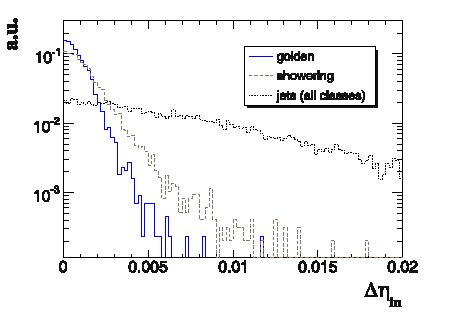
\includegraphics[width=0.45\linewidth]{Chapter04/Electrons/Images/elecs_deta.pdf}}\qquad
\subfloat[]{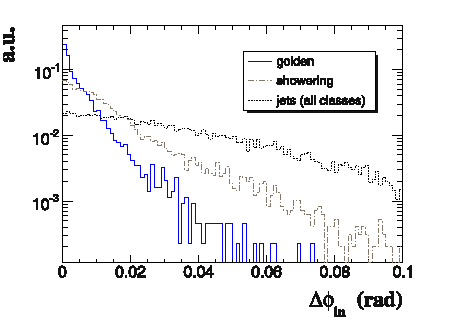
\includegraphics[width=0.45\linewidth]{Chapter04/Electrons/Images/elecs_dphi.pdf}}\\
\subfloat[]{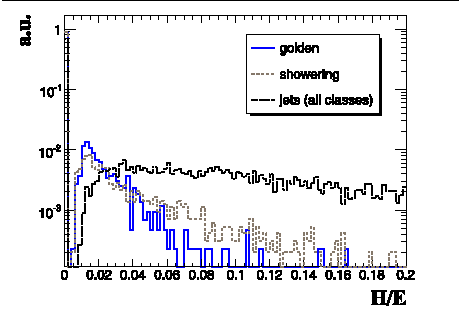
\includegraphics[width=0.45\linewidth]{Chapter04/Electrons/Images/elecs_hovere.pdf}}\qquad
\subfloat[]{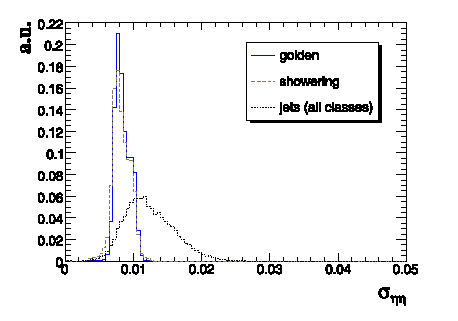
\includegraphics[width=0.45\linewidth]{Chapter04/Electrons/Images/elecs_sigmaietaieta.pdf}}
\caption[Distributions for the variables $\Delta\eta_{\text in}$, $\Delta\phi_{\text in}$, $\sigma_{i\eta i\eta}$ and $H/E$ for simulated electrons and misidentified jets.]{Distributions for (a) $\Delta\eta_{in}$, (b) $\Delta\phi_{in}$, (c) $H/E$ and (d) $\sigma_{i \eta i \eta}$. Here \textit{golden electrons} are those who emit minimal bremmstrahlung photons, \textit{showering} are electrons that lose a large faction of their energy in emissions and \textit{jets} are the typical distributions for hadronic jets.}
\label{FIGURE:PhysicsObjects_Electrons}
\end{figure}

\subsection{Veto electrons}

We define \textit{veto electrons} as an electron candidate with $\pt>10\,\GeV$ and $|\eta|<2.4$ which passes the \gls{CMS} Electron/Gamma \gls{POG} \cite{ARTICLE:CMSElectronReconstruction7TeV} requirements of the cut based electron \gls{ID} \textit{veto electron} working point. A summary of these conditions can be found in table \ref{TABLE:PhysicsObjects_ElectronPOG_CutBased_VetoElectronRequirements}.
 
\begin{table}[!htp]
\centering
\begin{tabular}{|l|c|c|}
\hline
Variable  $\pt > 20 (p_{T} <= 20)$ & Barel & Endcap \\
\hline\hline
$| \Delta\eta(track,supercluster) |$                           & $<0.004$ & $<0.005$ \\
$| \Delta\phi(track,supercluster) |$                           & $<0.3  $ & $<0.2  $ \\
$ \sigma(i\eta,i\eta)$                                         & $<0.01 $ & $<0.03 $ \\
$H/E$                                                          & $<0.12 $ & $<0.10 $ \\
\cline{2-3}
$|d_{0}(vertex)|$                                              & \multicolumn{2}{c|}{$<0.02\,\centi\meter$} \\
$|d_{Z}(vertex)|$                                              & \multicolumn{2}{c|}{$<0.1\,\centi\meter$}  \\
$|\frac{1}{E}-\frac{1}{p}| $                                   & \multicolumn{2}{c|}{$<0.05$} \\
\cline{2-3}
$\frac{PF_{isolation}}{p_{\perp}}$ for $ \Delta R_{cone}=0.3$ & $<0.10 $ & $<0.10(0.07)$ \\
\cline{2-3}
Conversion rejection: vertex fit probability                   & \multicolumn{2}{c|}{$<1 \times 10^{6}$}  \\
Conversion rejection: missing hits                             & \multicolumn{2}{c|}{$=0$} \\
\hline
\end{tabular}
\caption[Details of the CMS Electron-Gamma POG recommendations for a \textit{tight electron}.]
{Details of the CMS Electron-Gamma POG recommendations for a \textit{tight electron}. Here barrel is defined as $ |\eta_{supercluster}|<=1.479 $ and endcap is $ 1.479 < |\eta_{supercluster}| < 2.5 $.}
\label{TABLE:PhysicsObjects_ElectronPOG_CutBased_TightElectronRequirements}
\end{table}


\subsection{Tight electrons}

% More information at: 
%  * https://twiki.cern.ch/twiki/bin/viewauth/CMS/EgammaIDRecipes
%  * https://twiki.cern.ch/twiki/bin/view/CMS/EgammaCutBasedIdentification
%  * https://twiki.cern.ch/twiki/bin/view/CMS/EgammaEARhoCorrection

We also define \textit{tight electrons} as an electron candidate with $\pt>20\,\GeV$ and $|\eta|<2.4$ which passes the \gls{CMS} Electron/Gamma \gls{POG} requirements of the cut based electron \gls{ID} \textit{tight electron} working point. This working point is similar to the 2011 very tight WP70 working point. A summary of these conditions can be found in table \ref{TABLE:PhysicsObjects_ElectronPOG_CutBased_VetoElectronRequirements}.

\begin{table}[!htp]
  
\begin{tabular}{|l|c|c|}
\hline
Variable  $\pt > 20 (p_{\perp} <= 20)$ & Barel & Endcap \\
\hline\hline
$| \Delta\eta(track,supercluster) |$                           & $<0.004$ & $<0.005$ \\
$| \Delta\phi(track,supercluster) |$                           & $<0.3  $ & $<0.2  $ \\
$ \sigma(i\eta,i\eta)$                                         & $<0.01 $ & $<0.03 $ \\
$H/E$                                                          & $<0.12 $ & $<0.10 $ \\
\cline{2-3}
$|d_{0}(vertex)|$                                              & \multicolumn{2}{c|}{$<0.02\,\centi\meter$} \\
$|d_{Z}(vertex)|$                                              & \multicolumn{2}{c|}{$<0.1\,\centi\meter$}  \\
$|\frac{1}{E}-\frac{1}{p}| $                                   & \multicolumn{2}{c|}{$<0.05$} \\
\cline{2-3}
$\frac{PF_{isolation}}{p_{\perp}}$ for $ \Delta R_{cone}=0.3$ & $<0.10 $ & $<0.10(0.07)$ \\
\cline{2-3}
Conversion rejection: vertex fit probability                   & \multicolumn{2}{c|}{1e-6}  \\
Conversion rejection: missing hits                             & \multicolumn{2}{c|}{$<=0$} \\
\hline
\end{tabular}
\caption{Details of the \gls{CMS} Electron-Gamma \gls{POG} recommendations for a \textit{tight electron}. Here barrel is defined as $ |\eta_{supercluster}|<=1.479 $ and endcap is $ 1.479 < |\eta_{supercluster}| < 2.5 $.}
\label{TABLE:PhysicsObjects_ElectronPOG_CutBased_VetoElectronRequirements}
\end{table}


%%%%%%%%%%%%%%%%%%%%%%%%%%%%%%%%%%%%%%%%%%%%%%%%%%%%%%%%%%%%%%%%%%%%%%%%%%%%%%%%%%%%%%%
%%% SUBSECTION
%%%%%%%%%%%%%%%%%%%%%%%%%%%%%%%%%%%%%%%%%%%%%%%%%%%%%%%%%%%%%%%%%%%%%%%%%%%%%%%%%%%%%%%
\subsection{Isolation}
\label{SUBSECTION:EventReconstructionAndSimulation_LeptonIsolation_Isolation}

% More information
%  * https://twiki.cern.ch/twiki/bin/view/CMS/EgammaCutBasedIdentification#Detector_Isolation
%  * https://twiki.cern.ch/twiki/bin/view/CMS/EgammaEARhoCorrection#Isolation_cone_R_0_3

%Status: Writting

For electrons we calculate the \textit{effective area corrected isolation} over a cone of $\Delta R<0.3$ around the electron. For the neutral \gls{PU} subtraction we uses a look-up table of effective areas according to electron $|eta|$ which is multiplied by the estimated neutral \gls{PU} energy density by unit of effective area. The definition for this isolation can be found in equation \ref{EQUATION:ElectronIsolation}.

\begin{equation}
I = \sum^{\substack{\text{charged} \\ \text{non-pileup}}}\pT +
\text{max}\left(0,\sum^{\text{neutral}}\pT+\sum^{\text{photon}}\pT - \rho(\text{lepton}) \times \text{Eff. Area}(\text{lepton})\right)
\label{EQUATION:ElectronIsolation}
\end{equation}

For the \gls{VBF} Higgs to invisible Run I analysis we used the \gls{CMS} Electron/Gamma \gls{POG} recommend values together with our own minimum electron \pt requirements become $I_{rel}^{electron}<0.15$ for \textit{loose electron} working point and $I_{rel}^{electron}<0.10$ for the \textit{tight electron} working point.

%%%%%%%%%%%%%%%%%%%%%%%%%%%%%%%%%%%%%%%%%%%%%%%%%%%%%%%%%%%%%%%%%%%%%%%%%%%%%%%%%%%%%%%
%%% SECTION
%%%%%%%%%%%%%%%%%%%%%%%%%%%%%%%%%%%%%%%%%%%%%%%%%%%%%%%%%%%%%%%%%%%%%%%%%%%%%%%%%%%%%%%
\section{Muons}
\label{SECTION:EventReconstructionAndSimulation_Muons}

%Status: DONE

Muon track reconstruction starts independently at the inner-tracker (\textit{tracker track} and in the muon systems (\textit{standalone-muon track}) \cite{ARTICLE:CMSMuonReconstruction7TeV}. Then this information can be combined into a single muon track in two possible ways.

\textit{Global Muon reconstruction} is an \textit{outside-in algorithm}. We starts by finding tracker track match for each stand-alone muon track. This is done by propagating the match candidate pair to a common surface and comparing track parameters. For each matched pair, a \textit{global-muon fit} is performed using all hits from the two tracks using a Kalman-filter algorithm \cite{ARTICLE:KalmanFilteringTrackVertexFitting}. For muons of $\pt\gtrsim 200\,\GeV/c$, it has been showed that a \textit{global-muon fit} improves the momentum resolution compared to a \textit{tracker-only fit} \cite{CMSTDR:CMSPhysicsVol1, ARTICLE:CMSPerformanceMuonReconstructionCosmicRay}.

\textit{Tracker Muon reconstruction} is an \textit{inside-out algorithm}. In this method we start by selecting all tracker tracks with $\pt>0.5\,\GeV$ and $p>2.5\,\GeV$. We extrapolate those tracks to the muon system while taking into account the magnetic field, energy loss and scattering. If we find a match with at least one muon segment in the muon system (track stub in the \gls{DT} or \gls{CSC}) this this tracker track now becomes a Tracker Muon. 

Tracker muon reconstructions is more efficient than the global muon reconstruction at low momenta at $p\lesssim 5\,\GeV$. This difference is due to tracker muons reconstruction only requiring one segment on the muon system. While global muon reconstruction is more efficient for higher energies where the muons are more likely to pass several muon stations.

Muons can be also be classified as prompt of non-prompt. The prompt muons are the ones produced directly in the hard process like the decays of vector bosons or quarkonia particle decays. On the other hand, non-prompt muons typically come from in-flight decays light hadrons, from taus or heavy quark decays. 

When reconstructing global muons, its unlikely to find non-prompt muons but we may have hadronic activity ``punching-through'' the calorimeter system and appearing in the muon system. To reduce this types of background we can use different muon identification criteria. We can define a ``tight muon'' as global fit track using tracker and muon chamber hits with a $\chi^2$ per degree of freedom os less than 10. This fit must include at least one segment in the muon chamber, track segments in at least 2 muon stations, use more than 10 hits in the inner tracker of which at least one in the a pixel layer and finally a small transverse impact paramenter $|d_{xy}|< 2\,\milli\meter$. The efficiency for such a criteria has been measured both in data and Monte Carlo using $J/\psi \rightarrow \mu^+ \mu^-$ and $Z \rightarrow \mu^+ \mu^-$ and for $\pt > 10 \,\GeV$ it plateaus at 96-99\% \cite{ARTICLE:CMSMuonReconstruction7TeV}.

%%%%%%%%%%%%%%%%%%%%%%%%%%%%%%%%%%%%%%%%%%%%%%%%%%%%%%%%%%%%%%%%%%%%%%%%%%%%%%%%%%%%
%%% SUBSECTION
%%%%%%%%%%%%%%%%%%%%%%%%%%%%%%%%%%%%%%%%%%%%%%%%%%%%%%%%%%%%%%%%%%%%%%%%%%%%%%%%%%%%
\subsection{Loose Muons}

% From: https://twiki.cern.ch/twiki/bin/view/CMSPublic/SWGuideMuonId
%
% bool muon::isLooseMuon (const reco::Muon & recoMu);
% Particle-Flow muon id     & recoMu.isPFMuon()                               & Can be complemented by muon quality cuts similar to those used in the Tight Muon selection.
% Is Global OR Tracker Muon & recoMu.isGlobalMuon() || recoMu.isTrackerMuon() & Avoid using muons which are only Standalone Muons. (~0.01% of PF muons) 
% REFERENCE: MUO-10-004

We can define \textit{loose muon} using the cut based definitions recommend by the \gls{CMS} Muon \gls{POG} \cite{ARTICLE:CMSPerformanceOfMuonID7TeV} with the same name, where we require the muon candidate to be a \gls{PF} muon which is also a tracker or global muon. We exclude only standalone muons which are only $\approx 0.01\%$ of the \gls{PF} muons. Additionally we require the muon candidate to have $\pt>10\,\GeV$, $|\eta|<2.1$ and relative combined isolation $<0.2$.

%%%%%%%%%%%%%%%%%%%%%%%%%%%%%%%%%%%%%%%%%%%%%%%%%%%%%%%%%%%%%%%%%%%%%%%%%%%%%%%%%%%%
%%% SUBSECTION
%%%%%%%%%%%%%%%%%%%%%%%%%%%%%%%%%%%%%%%%%%%%%%%%%%%%%%%%%%%%%%%%%%%%%%%%%%%%%%%%%%%%
\subsection{Tight Muons}

We can also define \textit{tight muon} as a muon candidate which has $\pt>20\,\GeV$, $|\eta|<2.1$. It is an isolated muon passing relative Combined Isolation $<0.12$, And it is compatible with being produced at the primary vertex by requiring $d_{xy}<0.045\,\milli\meter$ and $d_z < 0.2\,\milli\meter$. We additionally require the muon to pass the  \gls{CMS} Muon \gls{POG} recommended cut based \textit{tight muon} identification criteria that requires the candidate to be a \glsreset{PF} muon which is also a global muon. Where the the global track fit has at least one muon chamber hit and $\chi^2/ndof < 10$. The presence of muon segments in at least two chambers. The numbers os tracker layers with hits needs to be more than five and we also require at least one pixel hit.

%%%%%%%%%%%%%%%%%%%%%%%%%%%%%%%%%%%%%%%%%%%%%%%%%%%%%%%%%%%%%%%%%%%%%%%%%%%%%%%%%%%%%%%
%%% SUBSECTION
%%%%%%%%%%%%%%%%%%%%%%%%%%%%%%%%%%%%%%%%%%%%%%%%%%%%%%%%%%%%%%%%%%%%%%%%%%%%%%%%%%%%%%%
\subsection{Isolation}
\label{SUBSECTION:EventReconstructionAndSimulation_LeptonIsolation_MuonsIsolation}

% More information:
%  * https://twiki.cern.ch/twiki/bin/view/CMSPublic/SWGuideMuonId#Muon_Isolation

%Status: DONE

For muons we use the \textit{combined isolation} over a cone of $\Delta R < 0.4$ around the muon. For neutral \gls{PU} subtraction we use the determined charged \gls{PU} component inside the cone and multiply it by a factor of 0.5 which is determined from simulation. The definition for this isolation can be found in equation \ref{EQUATION:MuonIsolation}.

\begin{equation}
I = \sum^{\substack{\text{charged} \\ \text{non-pileup}}}\pT +
\text{max}\left(0,\sum^{\text{neutral}}\pT+\sum^{\text{photon}}\pT-\frac{1}{2}\sum^{\substack{\text{charged}
\\ \text{pileup}}}\pT\right)
\label{EQUATION:MuonIsolation}
\end{equation}

For the \gls{VBF} Higgs to invisible Run I analysis we used the \gls{CMS} Muon \gls{POG} recommend \textit{Tight Isolation} working point of $I_{rel}^{muon}<0.12$.

%\cite{ARTICLE:CMSMuonReconstruction7TeV} %AG 72

%%%%%%%%%%%%%%%%%%%%%%%%%%%%%%%%%%%%%%%%%%%%%%%%%%%%%%%%%%%%%%%%%%%%%%%%%%%%%%%%%%%%%%%
%%% SECTION
%%%%%%%%%%%%%%%%%%%%%%%%%%%%%%%%%%%%%%%%%%%%%%%%%%%%%%%%%%%%%%%%%%%%%%%%%%%%%%%%%%%%%%%
\section{Jets}
\label{SECTION:EventReconstructionAndSimulation_Jets}

%Status: DONE

When we collide hadrons the most probable hard processes will produce quarks and gluons. However, these do not reach our detectors. They quickly hadronize and fragment generating a collimated spray of particles which is commonly referrer to as a jet. To determine the properties of this outgoing quarks and gluons we need therefore to look at the characteristics of their associated jets. To achieve this goal we need to combine the measured jet remnants in a way that preserves the physical properties of the original particle.

%%%%%%%%%%%%%%%%%%%%%%%%%%%%%%%%%%%%%%%%%%%%%%%%%%%%%%%%%%%%%%%%%%%%%%%%%%%%%%%%%%%%%%%
%%% SUBSECTION
%%%%%%%%%%%%%%%%%%%%%%%%%%%%%%%%%%%%%%%%%%%%%%%%%%%%%%%%%%%%%%%%%%%%%%%%%%%%%%%%%%%%%%%
\subsection{Jet Clustering}
\label{SECTION:EventReconstructionAndSimulation_Jets_JetClustering}

%Status: DONE

Jet clustering algorithms are sets of rules that allows us to combine a particle candidates into a jets \cite{ARTICLE:TowardsJetography}. These algorithms normally are controlled by parameters that define how close particles need to be in order to be associated into a jet and a way to combine their momentum. However, a jet definition should be robust and provide consistent measurements about the parton. There are two major families of problems that may affect a jet algorithms. These problems appear when the number of jets in an event changes by adding a soft collinear gluon emissions (collinear safety) or by parton splitting (infrared safety). 

In \gls{CMS} we used a sequential recombination algorithm known as anti-$k_T$ \cite{ARTICLE:AntiKtAlgorithm} which is both infrared and collinear safe. This algorithm starts be determining a measurement of distance between every pair of objects $d_{ij}$ and a the distance of each object to the beamline $d_{iB}$. The definition of this distances can be found in equations \ref{EQUATION:EventReconstructionAndSimulation_AKDistances1} and \ref{EQUATION:EventReconstructionAndSimulation_AKDistances2} respectively. 

\begin{align}
d_{ij} &= \text{min}({\pT}_{i}^{2p},{\pT}_{j}^{2p})\frac{\Delta R_{ij}^{2}}{R^{2}} \label{EQUATION:EventReconstructionAndSimulation_AKDistances1} \\
d_{iB} &= {\pT}_{i}^{2p}\ \label{EQUATION:EventReconstructionAndSimulation_AKDistances2} 
\end{align}

Where $\Delta R$ is the separation the $\eta-phi$ plane and $R$ is the maximum diameter for the jet. The parameter $p$ defines what type of algorithm we Choose. For $p$ is equal to 1 for the $k_T$ algorithm, 0 for the Cambridge/Aachen algorithm and -1 for the anti-$k_T$. 

After determining all the $d_{ij}$ and $d_iB$ we determine the minimum distance, if it is a $d_{ij}$ we combine those two object and recalculate all the distances. If the minimum is a $d_iB$ we declare $i$ to be a \textit{final state jet}, and remove it from the list of particles and recalculate all the again distances. The procedure continues until there are no more objects remaining.

The anti-$k_T$ algorithm tend to cluster particles around a the hardest particle in a region which normally leads to a cone like jet area in the $\Delta\phi$ plane. In the \gls{VBF} Higgs to invisible analysis the clustering is made over \gls{PF} particle candidates following the implementation in the \textsc{fastjet} software package \cite{ARTICLE:FastJetUserManual}. The \gls{CMS} recommended cone diameter size for 2012-13 analysis is of 0.5 while for 2015 is of 0.4.

%\cite{ARTICLE:TowardsJetography} %AG 76
%\cite{ARTICLE:AntiKtAlgorithm}   %AG 77
%\cite{ARTICLE:FastJetUserManual} %AG 78

%%%%%%%%%%%%%%%%%%%%%%%%%%%%%%%%%%%%%%%%%%%%%%%%%%%%%%%%%%%%%%%%%%%%%%%%%%%%%%%%%%%%%%%
%%% SUBSECTION
%%%%%%%%%%%%%%%%%%%%%%%%%%%%%%%%%%%%%%%%%%%%%%%%%%%%%%%%%%%%%%%%%%%%%%%%%%%%%%%%%%%%%%%
\subsection{Particle Flow Jet Identification} 
\label{SECTION:EventReconstructionAndSimulation_Jets_ParticleFlowJetID}

%Status: DONE

% More information at:
% https://twiki.cern.ch/twiki/bin/view/CMS/JetID

The \gls{CMS} Jet-MET \gls{POG} has defined criteria to reject fake, badly reconstructed and noisy \gls{PF} jets while keeping 98-99\% real jets. I all the analysis presented in this thesis we have used the recommended \gls{PF} jet \gls{ID} loose working point. We require all jets to have at least two constituents and both neutral hadron fraction and a neutral \gls{EM} fraction to be below 99\%. Additionally for jets inside the tracker acceptance with $|\eta| < 2.4$ we require the charged multiplicity and charged hadron fraction to be at bigger than zero and the charged \gls{EM} fraction to be less than 99\%.

%%%%%%%%%%%%%%%%%%%%%%%%%%%%%%%%%%%%%%%%%%%%%%%%%%%%%%%%%%%%%%%%%%%%%%%%%%%%%%%%%%%%%%%
%%% SUBSECTION
%%%%%%%%%%%%%%%%%%%%%%%%%%%%%%%%%%%%%%%%%%%%%%%%%%%%%%%%%%%%%%%%%%%%%%%%%%%%%%%%%%%%%%%
\subsection{Pileup Jet Identification}
\label{SECTION:EventReconstructionAndSimulation_Jets_PileupJetID}

%Status: DONE

% More information at:
% https://twiki.cern.ch/twiki/bin/view/CMS/PileupJetID

To identify if a \gls{PF} jet has come from \gls{PU} or from the primary vertex we make of a \gls{BDT}. This machine learning algorithm was trained with information about, the trajectory of the tracks associated with the jet, the jet shape and object multiplicity. In the presented analysis we have used the recommended loose working point of the \textit{full \gls{BDT} method}. This method was be applied to each jet which would only be accepted if the \gls{BDT} output score would pass the cuts defined on table \ref{TABLE:EventReconstructionAndSimulation_PileupJetIDFullBDTLooseWorkingPoint} depending on jet \pt and \eta.

\begin{table}[!htb]
\centering
\begin{tabular}{|c|c|c|}
\hline
Jet $p_{\perp}$ & Jet $|\eta|$ & $BDT_{score}$ \\
\hline \hline
$20 < p_{\perp} \leq 30$ & $|\eta| < 2.5$            & $> -0.80$ \\
$20 < p_{\perp} \leq 30$ & $2.50 \leq |\eta| < 2.75$ & $> -0.85$ \\
$20 < p_{\perp} \leq 30$ & $2.75 \leq |\eta| < 3.00$ & $> -0.84$ \\
$20 < p_{\perp} \leq 30$ & $3.00 \leq |\eta| < 5.00$ & $> -0.85$ \\
$30 < p_{\perp}$         & $|\eta| < 2.5$            & $> -0.80$ \\
$30 < p_{\perp}$         & $2.50 \leq |\eta| < 2.75$ & $> -0.74$ \\
$30 < p_{\perp}$         & $2.75 \leq |\eta| < 3.00$ & $> -0.68$ \\
$30 < p_{\perp}$         & $3.00 \leq |\eta| < 5.00$ & $> -0.77$ \\
\hline
\end{tabular}
\caption{Table of the minimum values of \textit{full \gls{BDT} method} score for a \gls{PF} to be accepted as coming from the \gls{PV} using a loose working point. Required minimum values have been binned in jet \pt and \eta.}
\label{TABLE:EventReconstructionAndSimulation_PileupJetIDFullBDTLooseWorkingPoint}
\end{table}

%%%%%%%%%%%%%%%%%%%%%%%%%%%%%%%%%%%%%%%%%%%%%%%%%%%%%%%%%%%%%%%%%%%%%%%%%%%%%%%%%%%%%%%
%%% SUBSECTION
%%%%%%%%%%%%%%%%%%%%%%%%%%%%%%%%%%%%%%%%%%%%%%%%%%%%%%%%%%%%%%%%%%%%%%%%%%%%%%%%%%%%%%%
\subsection{Lepton cleaning}
\label{SECTION:EventReconstructionAndSimulation_Jets_LeptonCleaning}

%Status: DONE

To avoid having leptons being miss reconstructed as jets we filter out all jets which are located at $\Delta R < 0.5$ to any veto electron or loose muons.

%%%%%%%%%%%%%%%%%%%%%%%%%%%%%%%%%%%%%%%%%%%%%%%%%%%%%%%%%%%%%%%%%%%%%%%%%%%%%%%%%%%%%%%
%%% SUBSECTION
%%%%%%%%%%%%%%%%%%%%%%%%%%%%%%%%%%%%%%%%%%%%%%%%%%%%%%%%%%%%%%%%%%%%%%%%%%%%%%%%%%%%%%%
\subsection{Jet Energy Corrections}
\label{SECTION:EventReconstructionAndSimulation_Jets_JetEnergyCorrections}

%Status: DONE???

When reconstructing a jet the clustered energy often does not match the parton energy that gave origin to the jet itself. There are many reason for this effect like non-linearity of the calorimeters response, detector noise, overlap with problematic detector areas, additional energy from \gls{PU}, miss calibration, etc. To fix this problem corrections are determined and applied to each jet in order to in average have energy measurements that are equal to the original hadron. This corrections can be factorized into components as it is represented in equation \ref{EQUATION:EventReconstructionAndSimulation_JetEnergyCorrections} \cite{ARTICLE:CMSDeterminationJetEnergyCalibration}.

\begin{equation}
P_{\text{corr}}^{\mu} = C_{\text{offset}}(\pT^{\text{raw}},\eta) \cdot C_{\text{rel}}(\pT^{\text{off}},\eta) \cdot C_{\text{abs}}(\pT^{\text{rel}},\eta) \cdot P_{\text{raw}}^{\mu}
\label{EQUATION:EventReconstructionAndSimulation_JetEnergyCorrections}
\end{equation}

The $C_{\text{offset}}$ term is accounts and subtracts the contribution of \gls{PU} and noise the the detector measurements. Its value is determined taking into account the specific event \pt-density express in the variable \rho, and the individual jet area A \cite{ARTICLE:PileupSubtractionJetAreas}. The event \rho is calculated as the median \pt-density of all jets present in the event. Since the median taken it will not be affected by the presence of hard jets. Unfortunately, the \glsreset{UE} activity has similar characteristic to the \gls{PU} and should not be subtracted. To avoid this the correction takes the form of $\rho - \langle \rho \rangle_{UE} \cdot A$, where $\langle \rho \rangle_{UE}$ is the average expected \gls{UE} contribution.

The $C_{\text{rel}}$ term is applied to make the energy response to be flat as a function of $\eta$. It is applied to the offset corrected transverse momentum $\pT^{off}$. To determine its value the \pt-balancing method is used \cite{ARTICLE:CMSDeterminationJetEnergyCalibration}. In this method we select a reference jet located in the central region where energy measurement is expected to be flat and a probe jet at any value of $\eta$. We can calculate the average of balance quantity as $(\pt^{\text{probe}} - \pt^{\text{reference}} ) / \pt^{\text{average}}$ which can be used to determine the correction to response in bins of jet \eta and dijet average \pt. 

The $C_{\text{abs}}$ term is intended to make the make the response uniform in \pt. It is applies to the $\pT^{rel}$ and is calculated using the \gls{MPF} method \cite{ARTICLE:CDFDijetAngularDistribution}. In this method we use the good \gls{CMS} resolution for leptons and photons in processes like $\gamma + \text{jets}$ and $Z + \text{jets}$ to infer on the properties of the recoil jets. Since this processes should have include missing energy if observed it can be used to calibrate the jet response for the jets present in the event.

%TODO: Check with patrick
The total uncertainty on the jet energy scale is obtained by summing in quadrature the estimated uncertainties of each one of the correction terms. For \gls{PU} jets the total uncertainty is in the range of 3-5\% depending on \pt and \eta \cite{ARTICLE:CMSDeterminationJetEnergyCalibration}.

% \cite{ARTICLE:CMSDeterminationJetEnergyCalibration} % AG 79
% \cite{ARTICLE:PileupSubtractionJetAreas}            % AG 80
% \cite{ARTICLE:CDFDijetAngularDistribution}          % AG 81

%%%%%%%%%%%%%%%%%%%%%%%%%%%%%%%%%%%%%%%%%%%%%%%%%%%%%%%%%%%%%%%%%%%%%%%%%%%%%%%%%%%%%%%
%%% SECTION
%%%%%%%%%%%%%%%%%%%%%%%%%%%%%%%%%%%%%%%%%%%%%%%%%%%%%%%%%%%%%%%%%%%%%%%%%%%%%%%%%%%%%%%
\section{Hadronic Taus}
\label{SECTION:EventReconstructionAndSimulation_Taus}

%Status: DONE

Taus can decay leptonically and hadronically. In leptonic decays the tau decays directly to an electron or and two additional neutrinos. Therefore it is very difficult to identify such decays experimentally. On the other hand an hadronic tau decay produces a characteristic signature of a narrow jet containing an odd number of charged particles and additional neutral hadrons, as well as a tau neutrino. The most frequent decay modes have one or three charged $\pi$ mesons and are summarized in table \ref{TABLE:EventReconstructionAndSimulation_TauDecays}. In all the analysis presented in this thesis when referring to a tau we refer an hadronically decaying tau.

\begin{table}[!htb]
\begin{tabular}{|l|c|r|r|}
\hline
Decay Channel & Resonance & Mass [$\MeV$] & Branching Fraction [\%] \\
\hline\hline
$\tau^{\pm} \rightarrow \pi^{\pm} \nu_\tau$                              &                &      & 11.6 \\
$\tau^{\pm} \rightarrow \pi^{\pm} \pi^{0}   \nu_\tau$                    & $\rho$         &  770 & 26.0 \\
$\tau^{\pm} \rightarrow \pi^{\pm} \pi^{0}   \pi^{0}   \nu_\tau$          & $\text{a}_{1}$ & 1260 & 10.8 \\
$\tau^{\pm} \rightarrow \pi^{\pm} \pi^{\mp} \pi^{\pm} \nu_\tau$          & $\text{a}_{1}$ & 1260 &  9.8 \\
$\tau^{\pm} \rightarrow \pi^{\pm} \pi^{\mp} \pi^{\pm} \pi^{0} \nu_\tau$  &                &      &  4.8 \\
\hline
Other hadronic modes                                                     &                &      &  1.7 \\
\hline\hline
Total & &  & 64.7 \\
\hline
\end{tabular}
\caption[Summary of the hadronic tau decay modes.]{Summary of the hadronic tau decay modes, with the branching fractions and intermediate resonances listed where relevant \cite{ARTICLE:PDG}.}
\label{TABLE:EventReconstructionAndSimulation_TauDecays}
\end{table}

Reconstruction of hadronic tau neutrinos with \gls{PF} is done by identifying the specific decay mode visible decay products. This approach is referred to as the \glsreset{HPS} algorithm \cite{ARTICLE:CMSPerformaceOfTauLeptonReconstruction,ARTICLE:CMSReconstructionIndentificationTau}. It combines reconstructed charged hadrons with strips of clustered photons which are interpreted as $\pi_0$. The reconstructed system is constrained by the tau mass and is highly collimated when compared with a typical \gls{QCD} jet. 

%%%%%%%%%%%%%%%%%%%%%%%%%%%%%%%%%%%%%%%%%%%%%%%%%%%%%%%%%%%%%%%%%%%%%%%%%%%%%%%%%%%%%%%
%%% SUBSECTION
%%%%%%%%%%%%%%%%%%%%%%%%%%%%%%%%%%%%%%%%%%%%%%%%%%%%%%%%%%%%%%%%%%%%%%%%%%%%%%%%%%%%%%%
\subsection{Hadron Plus Stips Algorithm}
\label{SECTION:EventReconstructionAndSimulation_Taus_HPSAlgorithm}

%Status: DONE
%TODO: Review this with Andrew.

The \gls{HPS} algorithm utilizes \gls{PF} candidates to reconstruct charged pions and photons resulting from neutral pions decay. These photon can convert in into electron-positron pairs in the tracker material. This factors are taken into consideration, as well as these products deflection in the magnetic field. It also attempts to find the intermediate resonances listed in table \ref{TABLE:EventReconstructionAndSimulation_TauDecays} has a handle to determine the possible tau decay channel. Since the tau neutrino present on all decays cannot be directly measured it is not taken into account.


We seed the algorithm with \gls{PF} anti-$k_T$ jets with $R = 0.5$ where $\pt>14\,\GeV$ and $|\eta|<2.5$. To search for the $\pi^{0}$ decay products we try to identify strips by clustering \gls{PF} electrons and photons with $\pt>0.5\,\GeV$. We start from the most energetic electromagnetic particle inside the jet area and make that the centre of our candidate strip. We look for other electromagnetic objects within a window of $\Delta\eta = 0.05$ and $\Delta\phi = 0.20$ of the centre of the strip. If any object is found it gets associated with the strip and its four-momentum gets recalculated. We repeat the procedure until we cannot find any more electromagnetic in the strip. If the final strip object has a mass compatible with a $\pi^{0}$, in the interval between $50-200\,\MeV$, and has $\pt > 2.5 GeV$ it is kept. We then start the next strip clustering with the highest \pt electron or gamma not already belonging to a strip.

The charged pion candidates are required to have $\pt > 0.5\,\GeV$ and its track pass $d_z < 0.4\,\centi\meter$ and $d_{xy} < 0.03\,\centi\meter$ to the vertex associated with the highest \pt track in the jet, which is assumed to be the \tau production vertex.

The following topologies are taken into account by the \gls{HPS} algorithm:

\begin{enumerate}
  \item \textit{single hadron}: tries to identify tau decays into $\pi^{\pm} \nu_\tau$ or $\pi^{\pm} \pi^{0} \nu_\tau$ where the netral pion decay cannot be identified as a strips.
  \item \textit{One hadron + one strip}: tries to identify tau decays into $\pi^{\pm} \pi^{0} \nu_\tau$ where the $\pi^{0}$ decay photons are close together. The mass of the reconstructed $\tau_had$ is required to be in the interval $0.4<m_{\tau_had}<1.3\,\GeV$ for $\pt^{\tau_{had}} < 200\,\GeV$. The upper limit in the mass window can go up to $2.1\,\GeV$ for candidates with $\pt^{\tau_{had}} > 200\,\GeV$ to account for resolution effects.
  \item \textit{One hadron + two strip}: tries to identify tau decays into $\pi^{\pm} \pi^{0} \pi^{0} \nu_\tau$ where the $\pi^{0}$ decay photons are well separated. The mass of the reconstructed $\tau_had$ is required to be in the interval $0.4<m_{\tau_had}<1.2\,\GeV$ for $\pt^{\tau_{had}} < 200\,\GeV$. The upper limit in the mass window can go up $2.0\,\GeV$ and the $\pt^{\tau_{had}}$ increases above $200\,\GeV$.
  \item \textit{Three hadrons}: tries to identify tau decays into $\pi^{\pm} \pi^{\mp} \pi^{\pm} \nu_\tau$. The hadrons are required to have nass in the interval $0.8-1.5\,\GeV$ since we assume the $a_{1}$ intermediate resonance. Total charged is required to be one.
\end{enumerate}

There is no dedicated search for $\pi^{\pm} \pi^{\mp} \pi^{\pm} \pi^{0} \nu_\tau$ or higher pion multiplicity decay modes. These topologies are reconstructed with the currently defined criteria.

All selected hadrons and strips are required to be inside of cone of $\Delta R < 2.8\,\GeV/\pt^{\tau_{had}}$. The cone size is is constrained to the interval $\Delta R=0.05-0.10$. 

%%%%%%%%%%%%%%%%%%%%%%%%%%%%%%%%%%%%%%%%%%%%%%%%%%%%%%%%%%%%%%%%%%%%%%%%%%%%%%%%%%%%%%%
%%% SUBSECTION
%%%%%%%%%%%%%%%%%%%%%%%%%%%%%%%%%%%%%%%%%%%%%%%%%%%%%%%%%%%%%%%%%%%%%%%%%%%%%%%%%%%%%%%
\subsection{Isolation and Discriminants}
\label{SECTION:EventReconstructionAndSimulation_Taus_IsolationAndDiscriminants}

%STATUS: DONE

Isolation for taus is calculates in a similar way to electrons ans muons. The isolation variable is defined by summing the \pt of all \gls{PF} hadron and photon candidates in a cone of $\Delta R < 0.5$ around the tau axis. Here the charged hadron tracks are required to have $d_z < 2\,\milli\meter$ to the tau production vertex. We can subtract the contribution to isolation coming from \gls{PU} estimating its density in a cone of $\Delta R < 0.8$ around the tau and considering track with $d_z > 2\,\milli\meter$. All tau constituents are ignores on this sums. Working points have been defined for loose, medium and tight isolation \cite{ARTICLE:CMSReconstructionIndentificationTau}. 

Electrons can be reconstructed as taus when they make isolated deposits in the calorimeter or emit enough energy via bremmstrahlung to form a strip. A \gls{BDT} has been trained with a set of variables similar to the ones used in electron identification to exclude such miss reconstructions. In the \gls{CMS} Higgs to invisible analysis we use the tight working point.

Muons are less likely to be reconstructed as a tau. We can exclude such tau candidates by requiring that the track of the leading charged hadron is not also a tracker muon. This discriminator also has three possible working points, in our analysis we used the tight working point.

We can now define an hadronic tau candidate as a \gls{PF} tau candidates with $\pt > 20 \,\GeV$, $|\eta|<2.3$ and $d_z<0.2 \,\centi\meter$ to the primary vertex. We require that the candidate passes decay-mode identification, tight isolation and finally tight discriminators against electrons and muons.

%%%%%%%%%%%%%%%%%%%%%%%%%%%%%%%%%%%%%%%%%%%%%%%%%%%%%%%%%%%%%%%%%%%%%%%%%%%%%%%%%%%%%%%
%%% SECTION
%%%%%%%%%%%%%%%%%%%%%%%%%%%%%%%%%%%%%%%%%%%%%%%%%%%%%%%%%%%%%%%%%%%%%%%%%%%%%%%%%%%%%%%
\section{Missing Transverse Energy}
\label{SECTION:EventReconstructionAndSimulation_MET}

%Status: DONE

The Standard Model describes neutrinos as particles which only interact via the weak force. They can pass through our detectors without interacting and therefore not allowing any direct measurement. Many new models describe additional particles that would also be able to escape detection by leaving very small or no energy deposits in our experiments. The appearance of such particles can only be inferred through the measurement of an imbalance of transverse momentum of all detected particles. These effect can be quantified as the negative sum off all visible particle candidates transverse momentum in an event. 

The magnitude of that vector is referred to as \glsreset{MET}. Particle flow methodology provides a complete list of objects candidates in the event with excellent resolution achieved by combining all available information. It is the well suited to be the input for \gls{MET} calculation. Although \gls{CMS} has an excellent individual particle resolution the calculation of \gls{MET} is affected by the combined resolution of the measurement of all particles in the event. Figure \ref{FIGURE:EventReconstructionAndSimulation_METDistributionZmumu} shows the distribution for \gls{PF} \gls{MET} for both data and simulation for the selections of events of $Z \rightarrow \mu\mu$ and $\gamma +jets$ processes at $\sqrt{s}=8\,\TeV$. 

\begin{figure}[!htp]%
\centering
\subfloat[]{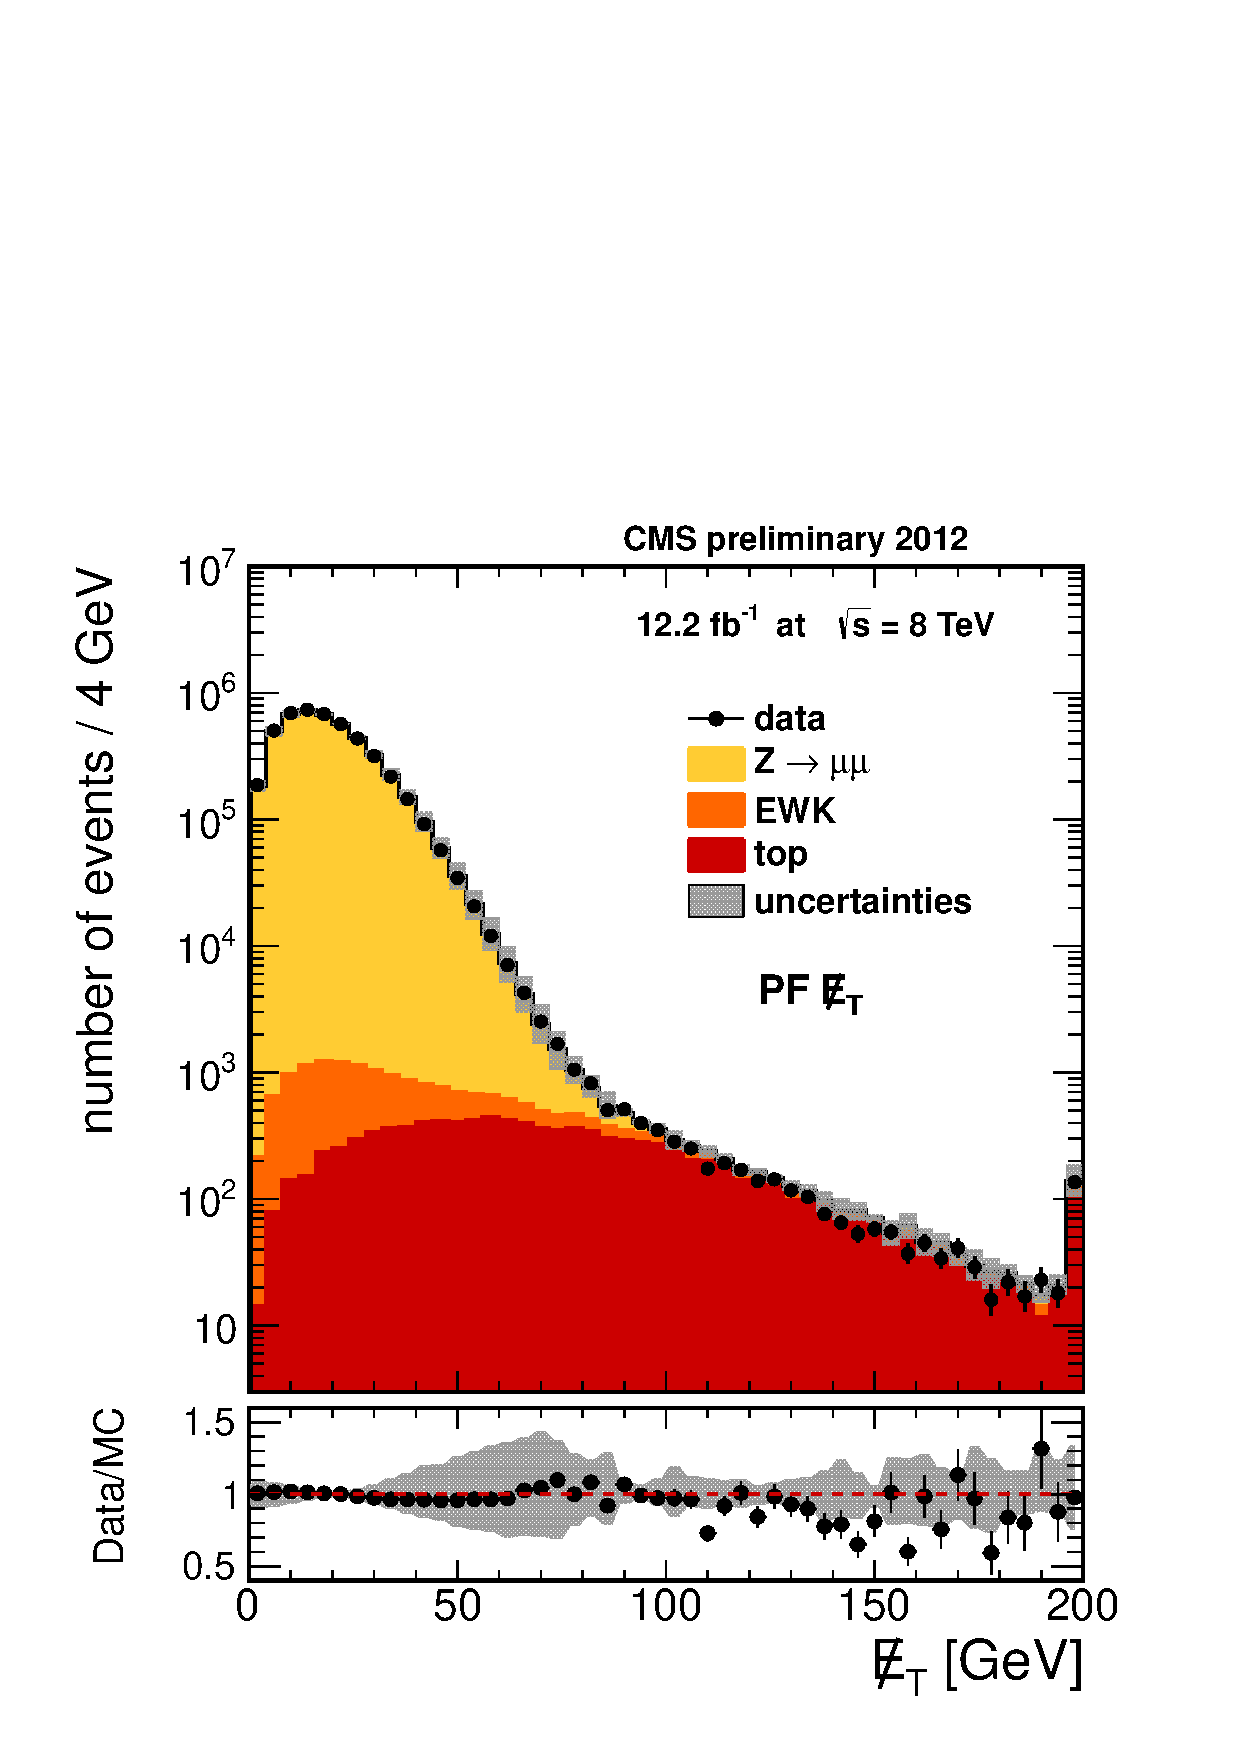
\includegraphics[width=0.45\textwidth]{Chapter04/MET/Images/met_zmm.pdf}}\qquad
\subfloat[]{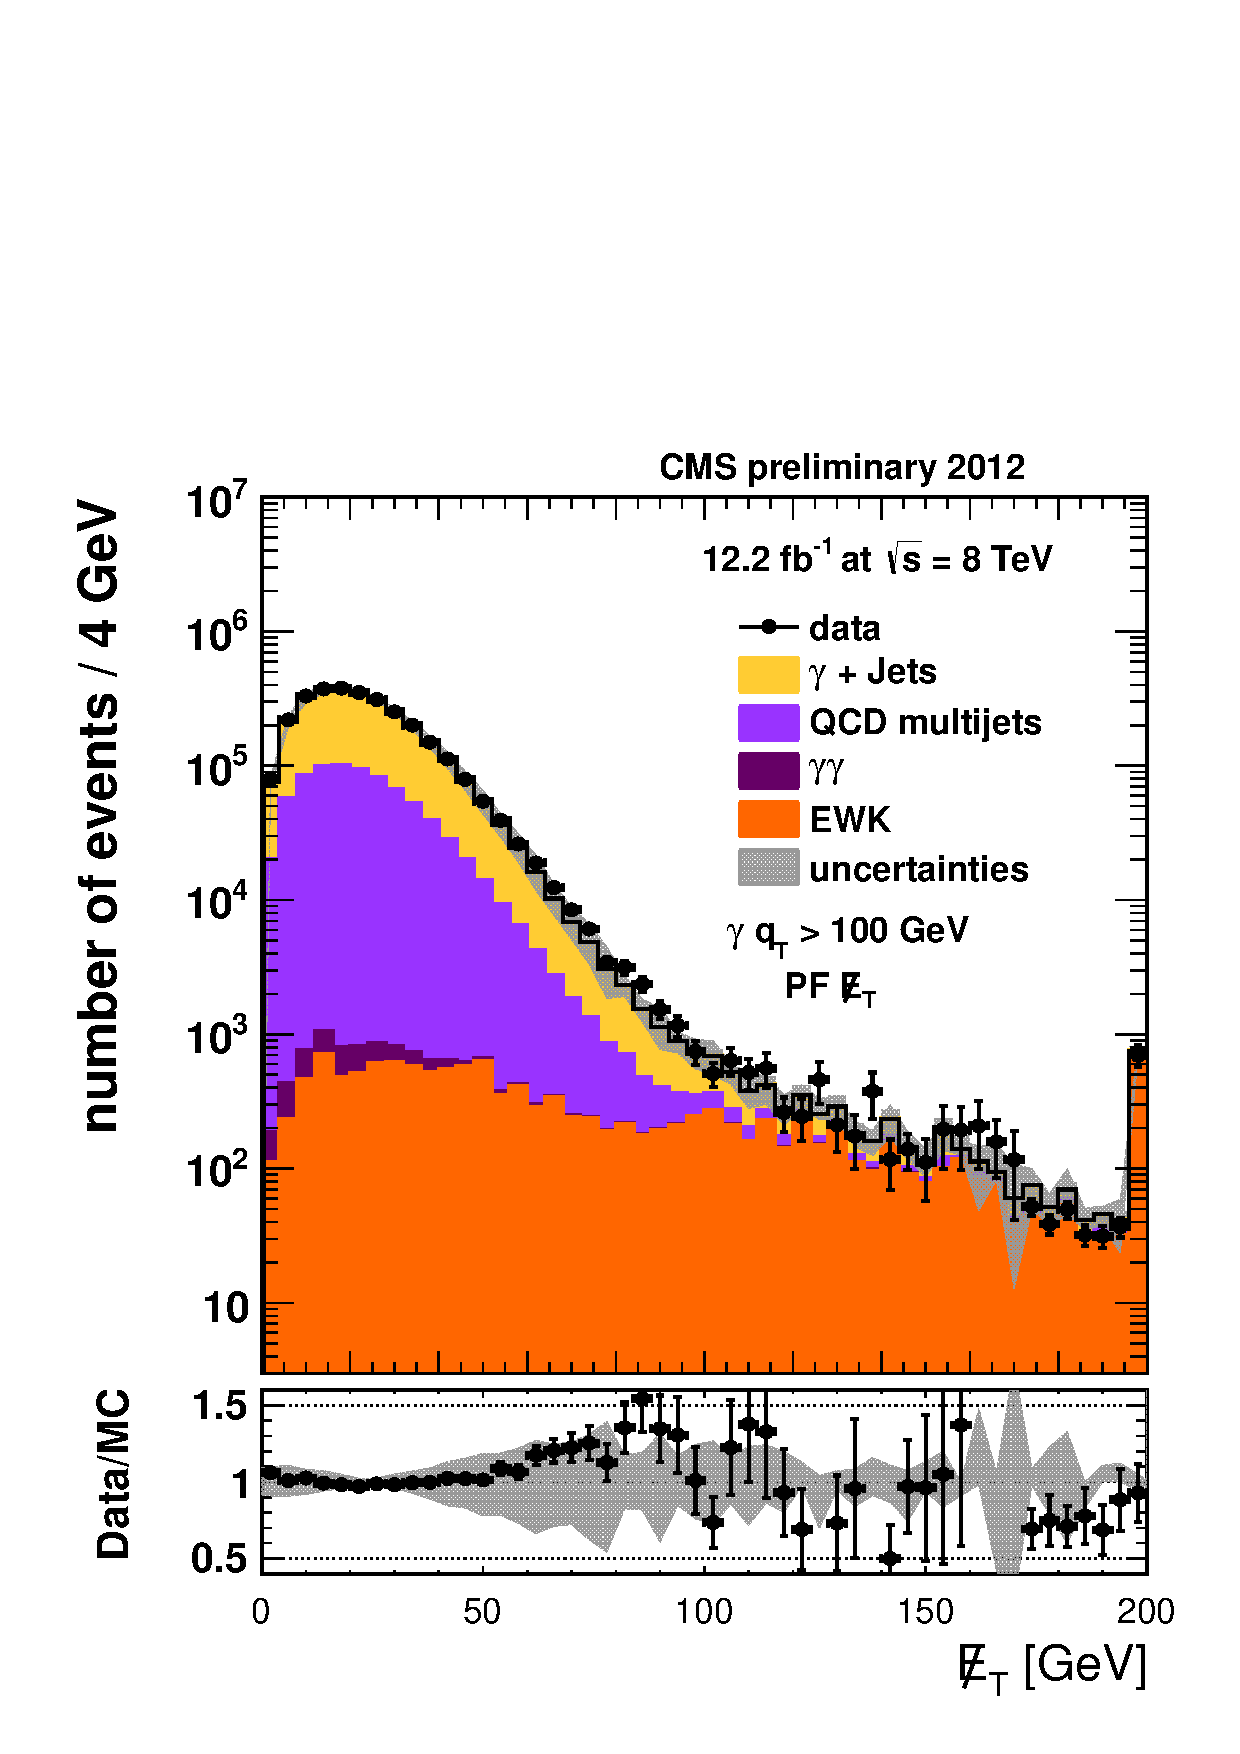
\includegraphics[width=0.45\textwidth]{Chapter04/MET/Images/met_gamma.pdf}}\\
 \caption[Distributions of the particle flow $\MET$ in $Z\rightarrow\gamma\gamma$ and $\gamma$+jets events in $\sqrt{s}=8\,\TeV$ data and simulation.]{Distributions of the particle flow $\MET$ in a) $Z\rightarrow\gamma\gamma$ and b) $\gamma$+jets events in $\sqrt{s}=8\,\TeV$ data and simulation. The uncertainty in the muon, photon, jet and neutral hadron energy responses is showed by the shaded band \cite{ARTICLE:CMSMETPerformance8TeV}.}
\label{FIGURE:EventReconstructionAndSimulation_METDistributionZmumu}
\end{figure}

Both photons and muons energy measurements have good resolution in the \gls{CMS} experiment and this processes do not involve real \gls{MET}. The observed distribution in both figures are predominantly shaped by the energy resolution of jet energy measurement.

During data taking issues with the detector or data acquisition can happen which create anomalously high \gls{MET} rendering this events unusable. The groups responsible for each part of the detector and physics object check the data after it was taken and to find if such problems occurred. After this problems are identified they produce software event filters fir analysts to be able to remove this problematic events. For analysis of 2012 data the \gls{CMS} JET-MET \gls{POG} working group recommended the use of filters to remove events affected by energy deposits from beam halo, noise in \gls{HCAL} readout electronics, particles directly hitting the \gls{ECAL} photodiodes, track reconstruction problems and finally \gls{ECAL} and \gls{HCAL} miss timed laser calibration sequence. This filters have been used in both prompt and parked \gls{VBF} Higgs to invisible analyses.

There are many factors that affect \gls{MET} response and resolution. These include zero suppression thresholds which dictate the minimum energy a calorimeter cell will report, dead or non-instrumented regions of the detector and reconstruction inefficiencies. Techniques have been developed to correct both response end resolution when using \gls{PF} \gls{MET} \cite{ARTICLE:CMSMissingTransverseEnergyPerformance}. These corrections include accounting for the bias in response due to using incorrect energy scale of the jets, and reducing the impact of pileup on the resolution \cite{ARTICLE:CMSMETPerformance8TeV}.

In the \gls{VBF} Higgs to invisible analysis we calculate and use \gls{MET} with our including muons. The variable is used in the offline analysis and trigger. This choice allows to investigate the irreducible background of $Z \rightarrow \nu\nu$ by using $Z \rightarrow \mu\mu$ as a proxy.

% \cite{ARTICLE:CMSMETPerformance8TeV}                 % AG 83
% \cite{ARTICLE:CMSMissingTransverseEnergyPerformance} % AG 84

%%%%%%%%%%%%%%%%%%%%%%%%%%%%%%%%%%%%%%%%%%%%%%%%%%%%%%%%%%%%%%%%%%%%%%%%%%%%%%%%%%%%%%%
%%% SECTION
%%%%%%%%%%%%%%%%%%%%%%%%%%%%%%%%%%%%%%%%%%%%%%%%%%%%%%%%%%%%%%%%%%%%%%%%%%%%%%%%%%%%%%%
\section{Monte Carlo Simulation}
\label{SECTION:EventReconstructionAndSimulation_MonteCarloSimulation}

\glsreset{MC} methods are a class of computer algorithms that rely on random sampling to obtain numerical results. This type of methods is especially useful in problems with many coupled degrees of freedom where it is difficult to perform analytical calculations. In particle physics these methods are often used to simulate physics processes, their interaction with detectors and the obtained measurements.

To simulate one event on the \gls{CMS} experiment we first start by the physics process itself. We can split this into two sub-processes: hard scattering and hadronization. There are many purpose built software programs that will perform each of these steps. An illustration of how the simulation of proton-proton collision is done with \gls{MC} programs can be found in figure \ref{FIGURE:EventReconstructionAndSimulation_MCShower}. A review of the available generators for \gls{LHC} physics can be found in \cite{ARTICLE:GeneralPurposeEventGeneratorsForLHCPhysics}.

\begin{figure}[!htb]
\centering
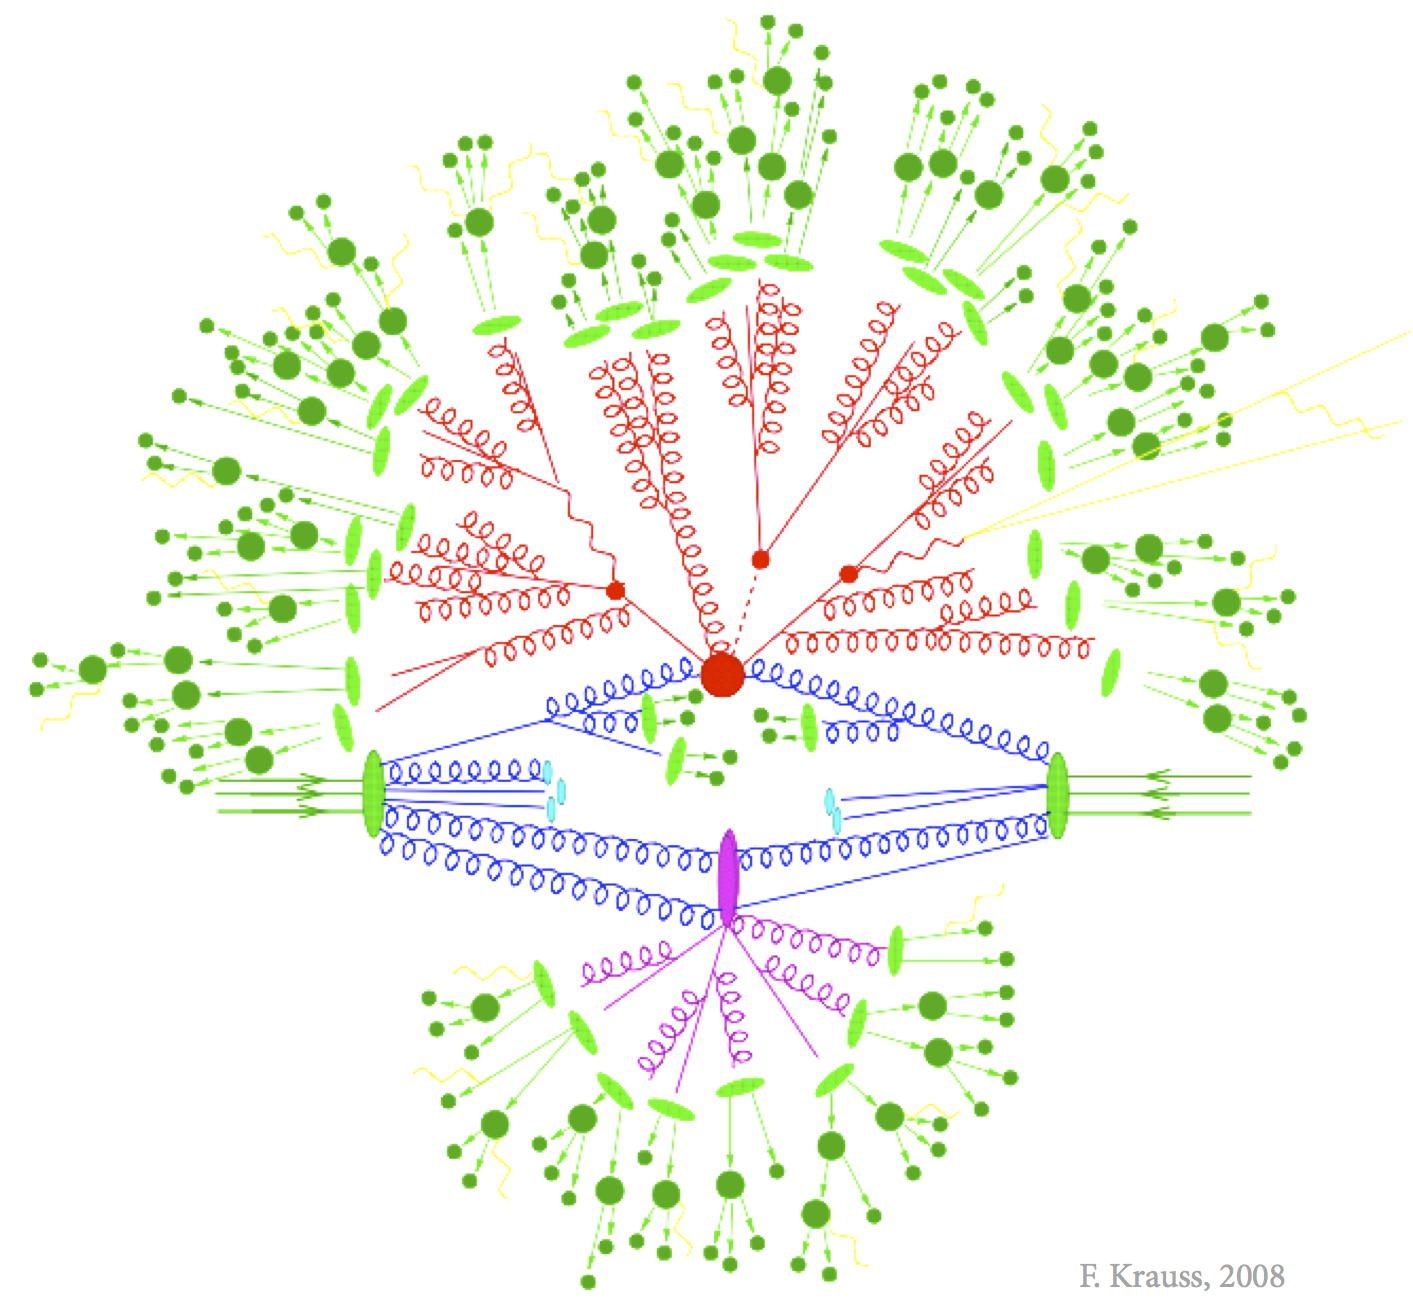
\includegraphics[width=0.8\textwidth]{Chapter04/MonteCarlo/Images/MCShower.png}
\caption[Illustration a proton-proton collision as implemented in MC event generators.]{Illustration of a proton-proton collision as implemented in some MC event generators \cite{IMAGEREF:krauss-diag}. Sub-processes are represented, the hard-scattering in the center of the diagram, the parton showering in red, hadronization in green. We can also observe the \gls{UE} interaction and its showering in purple.}
\label{FIGURE:EventReconstructionAndSimulation_MCShower}
\end{figure}

General purpose particle physics event generators like \textsc{PYTHIA 8} \cite{ARTICLE:Pythia6p4PhysicsAndManual,ARTICLE:Pythia8p1Introduction}, \textsc{HERWIG++} \cite{ARTICLE:HERWIGPhysicsAndManual} and \textsc{SHERPA} \cite{ARTiCLE:SherpaEventGenerator} are able to do both hard scattering and hadronization steps for a wide variety of physics processes. Typically these programs are restricted to $2 \rightarrow 2$ and $2 \rightarrow 1$ hard processes calculated at \gls{LO}.

There are many other dedicated matrix-element generators, like \textsc{MADGRAPH 5} \cite{ARTICLE:MadGraph5}, \textsc{ALPGEN} \cite{ARTICLE:ALPGENGenerator} and also \textsc{SHERPA} that focus on the hard process simulation. These programs provide $2 \rightarrow X$ hard scattering where a higher number of partons in the final state is possible. Some generators have also implemented \gls{NLO} calculations, which provide a better kinematics discription and lower uncertainties. Two examples of such generators are \textsc{aMC@NLO} \cite{ARTICLE:aMCatNLO} and \textsc{POWHEG} \cite{ARTICLE:POWHEG_2007,ARTICLE:POWHEG_2011}. This parton level events then need to be passed to a one of the general purpose event generators for hadronization. 

We need to avoid overlapping in the phase-space description of matrix-element and showering programs when simulating multi-jets events. The overlap comes from software like \textsc{PYTHIA} or \textsc{HERWIG} describing parton radiation as a Markov Chain process based on Sudakov form factors. This approach is only formally correct in the limit of soft and collinear emissions. On the other hand \gls{ME} programs like \textsc{MadGraph} works well for the hard scattering but diverges when the partons become soft or collinear. 

There are a few jet-parton matching schemes developed to account for this overlap \cite{ARTICLE:MatchingPartonShowersAndMatrixElements}. Showering can be vetoed and the event reweighed according like in the CKKW scheme \cite{ARTICLE:CKKWSchemeRef1,ARTICLE:CKKWSchemeRef2,ARTICLE:CKKWSchemeRef3} or events can be rejected altogether like in the MLM scheme \cite{ARTICLE:MLMScheme}. Depending on the generator used for the showering, different schemes are implemented and care must be taken in the definition of the matching parameters.

Most event generators can be finely tuned so all aspects of the simulation can be adjusted to experimental conditions. As consequence, in the \gls{CMS} experiment \textsc{PYTHIA} is used with the Z2 tune, which was produced using measurements made using minimum bias data at the Tevatron and \gls{LHC} \cite{ARTICLE:CMSMeasurementUnderlyingEventActivity}.  

After the physics event is simulated, the interaction with the detector and the corresponding electronics response is estimated using a precise model of the experiment. In the \gls{CMS} experiment \textsc{GEANT 4} \cite{ARTICLE:GEANT4ASimulationToolkit,ARTICLE:Geant4DevelopmentsAndApplications} software is used for this task which also relies heavily on \gls{MC} methods.




